% \AtBeginSection[]{
%     \begin{frame}
%         \frametitle{}
%         \tableofcontents[currentsection]
%     \end{frame}
% }

%%%%%%%%%%%%%%%%%%%%%%%%%%%%%%%%%%%%

\section{Preuve de Concept sur exemple}

\begin{frame}[fragile]{Preuve de Concept sur exemple}{Initialisation}

    \begin{columns}

        \begin{column}{0.6\textwidth}

            \begin{enumerate}
                \item Initialiser environment PettingZoo
                \item Mapping observation labels
            \end{enumerate}
    
\begin{lstlisting}[language=Python,basicstyle=\scriptsize]
from custom_envs.movingcompany import moving_company_v0
from prahom_wrapper.prahom_wrapper import prahom_wrapper

env = moving_company_v0.parallel_env(render_mode="human")

label_to_obs = {
    "empty_corridor_0": [0,1,0,0,1,0,0,1,0],
    "empty_corridor_1": [0,1,0,0,2,0,0,1,0],
    "empty_corridor_2": [0,1,0,0,3,0,0,1,0],
}
\end{lstlisting}
    
        \end{column}
    
        \begin{column}{0.4\textwidth}
            \centering
            \begin{figure}
                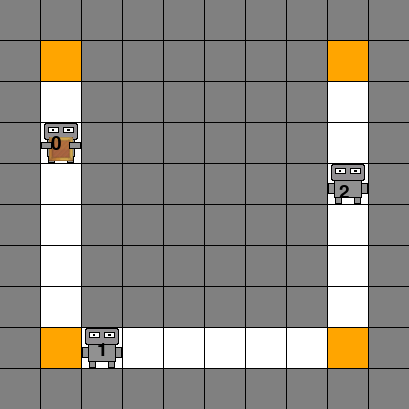
\includegraphics[width=\linewidth]{figures/moving_company_v0.png}
                \caption{Exemple de rendu graphique de l'environment \textquote{Moving Company}}
            \end{figure}
        \end{column}
    
    \end{columns}


\end{frame}


\begin{frame}

    % Boucle pour afficher toutes les images de frame000.png à frame099.png
    \foreach \i in {00, 01, 02, 03, 04, 05, 06, 07, 08, 09, 10, 11, 12, 13, 14, 15, 16, 17, 18, 19, 20} {
    
        \begin{onlyenv}<\i>
        % \begin{frame}[plain]
            \frametitle{Exemple : Moving Company après entrainement}
            \centering
            \includegraphics[width=0.5\textwidth]{figures/mcy_frames/frame_\i_delay-0.01s.png}
        % \end{frame}
    
        \end{onlyenv}
    
    }
    
\end{frame}


\begin{frame}[fragile]{Preuve de Concept sur exemple}{}

    \begin{columns}

        \begin{column}{0.6\textwidth}
    
            \textbf{Phase 1 : Modélisation}
    
            \begin{itemize}
                \item Développer manuellement un environnement simulé ($1.1$) où les agents doivent coopérer pour atteindre un objectif ($1.2$);
                \item Peut définir le comportement attendu des rôles sous forme d'historiques;
                \item Peut contraindre les agents à des rôles ($1.3$).
            \end{itemize}
    
            \begin{lstlisting}[language=Python,basicstyle=\scriptsize]
org_model = organizational_model(
    structural_specifications=ss(
        roles={ "role_0": history_subset(pattern="[o0,a1](1,4),[o1,a2](1,2)")},
        role_inheritance_relations=None, root_groups=None),
    
    functional_specifications=fs(
        social_scheme=sch(
            goals={"goal_0": history_subset(pattern="[#Any](0,*),[obs_goal_0]")},missions=["mission_0"], goals_structure=None,mission_to_goals={"mission_0": ["goal_0"]},mission_to_agent_cardinality=None),
        social_preferences=None),

    deontic_specifications={
        "role_0": {("mission_0", "Any"): ["agent_0", "agent_2"]}})\end{lstlisting}

        \end{column}
    
        \begin{column}{0.4\textwidth}
            \centering
            \adjustbox{trim={0.\width} {0.82\height} {0.\width} {0.\height}, clip}{%
                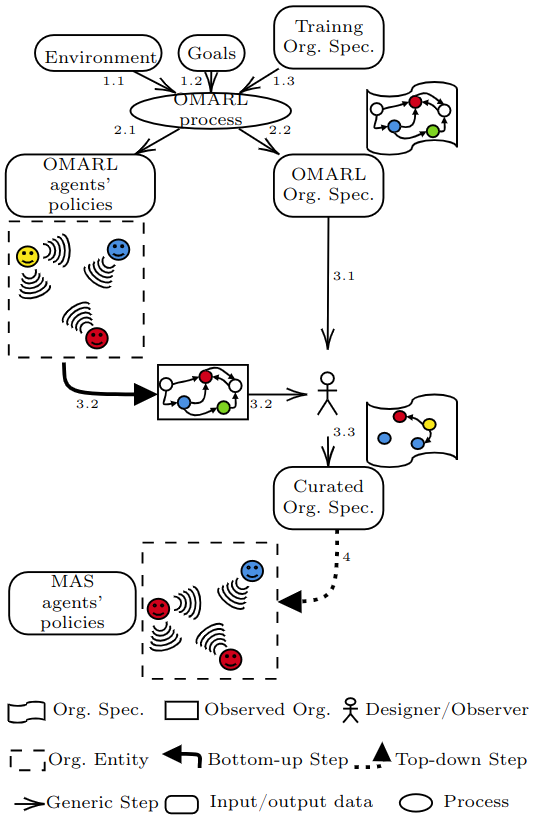
\includegraphics[width=1.2\linewidth]{figures/AOMEA_illustrative_view}
            }
        \end{column}
    
    \end{columns}
    
    
    \end{frame}
    
    
    \begin{frame}[fragile]{Preuve de Concept sur exemple}{}
    
    \begin{columns}
    
        \begin{column}{0.6\textwidth}
    
            \textbf{Phase 2 : Résolution}
    
            \begin{itemize}
                \item Algorithme MARL orienté organisation (OMARL) : processus MARL enrichi avec le modèle organisationnel;
                \item Résoudre en respectant les historiques contraints des rôles ($2.1$);
                \item Obtient l'OS associé ($2.2$)
            \end{itemize}

            \begin{lstlisting}[language=Python,basicstyle=\scriptsize]
pz_env.train_under_constraints(
    obs_act_to_labels=oal,
    constraint_integration_mode="CORRECT",algorithm_configuration="default_MAPPO"
    osh_model_constraint=osh_model)
            \end{lstlisting}

        \end{column}
    
        \begin{column}{0.4\textwidth}
            \centering
            \adjustbox{trim={0.\width} {0.56\height} {0.\width} {0.\height}, clip}{%
                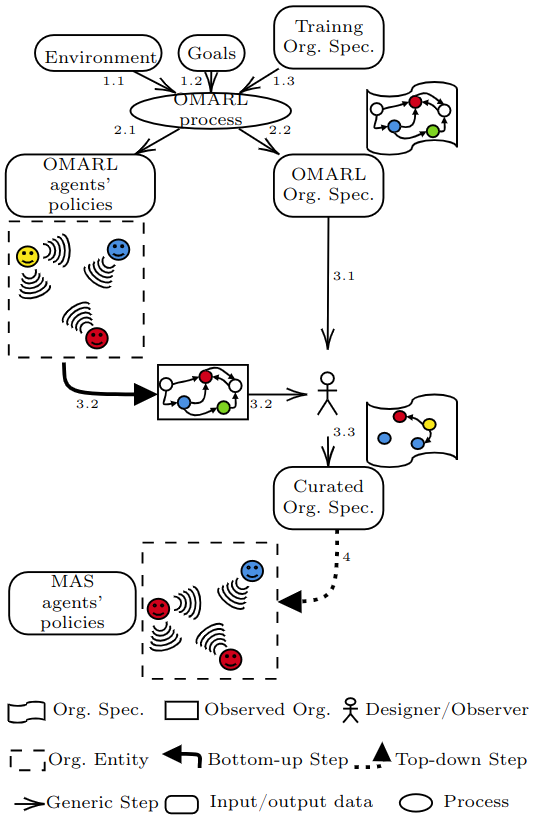
\includegraphics[width=1.2\linewidth]{figures/AOMEA_illustrative_view}
            }
        \end{column}
    
    \end{columns}
    
    \end{frame}
    
    \begin{frame}[fragile]{Preuve de Concept sur exemple}
    
    \begin{columns}
    
        \begin{column}{0.6\textwidth}
    
            \textbf{Phase 3 : Analyse}
    
            \begin{itemize}
                \item Les concepteurs observent les politiques des agents entraînés ($3.2$);
                \item Les concepteurs observent les SO calculés ($3.1$) : comprendre comment ils atteignent l'objectif;
                \item Les concepteurs obtiennent des indications de conception pour un SMA atteignant l'objectif : OS corrigé ($3.3$).
            \end{itemize}

            \begin{lstlisting}[language=Python,basicstyle=\scriptsize]
pz_env.generate_organizational_specifications(use_kosia=False, use_gosia=True,gosia_configuration={"generate_figures": True})
            \end{lstlisting}

        \end{column}
    
        \begin{column}{0.4\textwidth}
            \centering
            \adjustbox{trim={0.\width} {0.35\height} {0.\width} {0.188\height}, clip}{%
                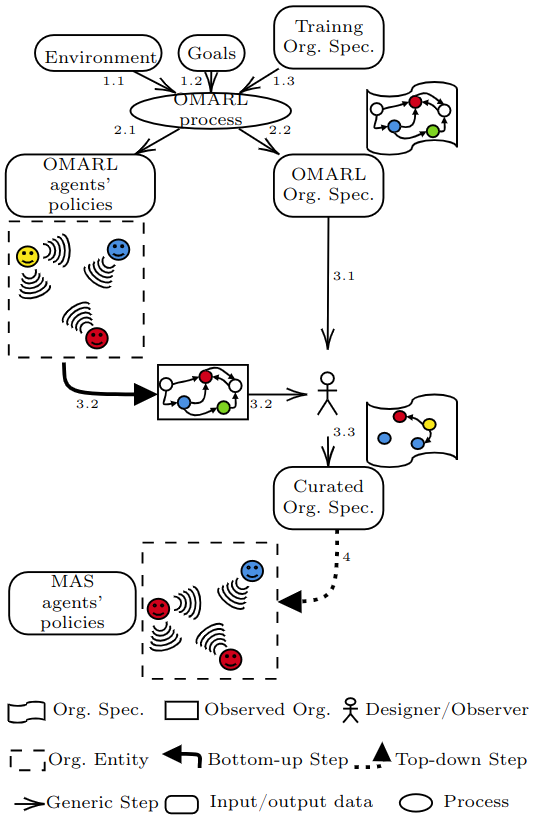
\includegraphics[width=1.2\linewidth]{figures/AOMEA_illustrative_view}
            }
        \end{column}
    
    \end{columns}
    
    \end{frame}
    
    \begin{frame}[fragile]{Preuve de Concept sur exemple}

        \begin{figure}
            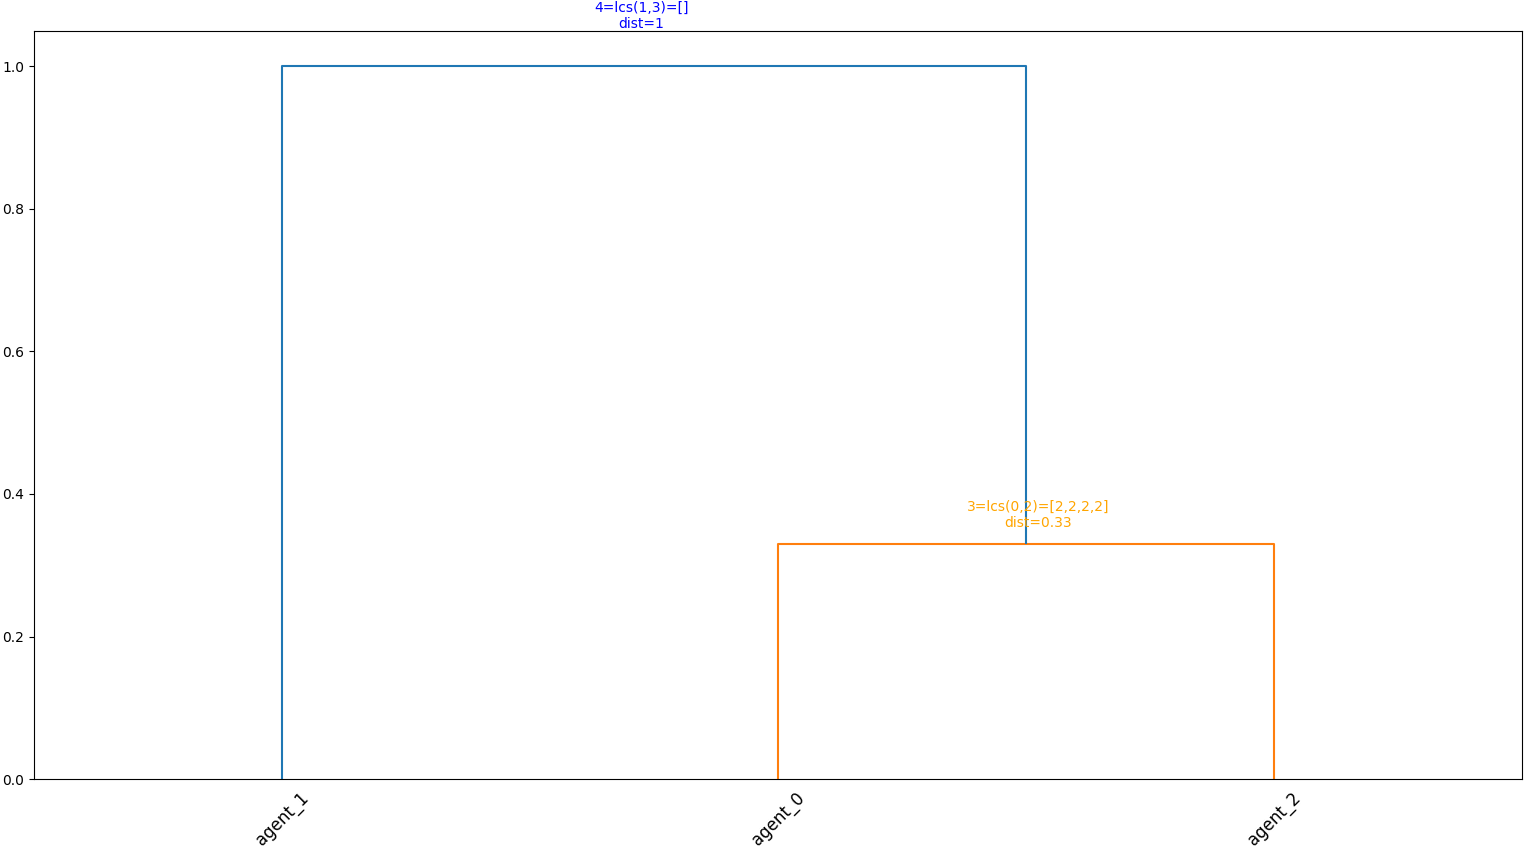
\includegraphics[width=0.7\linewidth]{figures/role_clustering.png}
            \caption*{Exemple de Dendrogramme obtenu après \textit{Hierarchical Clustering}}
        \end{figure}

    \end{frame}
        

    \begin{frame}[fragile]{Preuve de Concept sur exemple}
    
    \begin{columns}
    
        \begin{column}{0.6\textwidth}
    
            \textbf{Phase 4 : Développement}
    
            \begin{itemize}
                \item Les concepteurs observent l'OS corrigé pour implémenter un SMA;
                \item Développement d'un SMA régulier, traitant ainsi les questions de sécurité;
                \item Évaluation du SMA implémenté dans des simulations.
            \end{itemize}
    
        \end{column}
    
        \begin{column}{0.4\textwidth}
            \centering
            \adjustbox{trim={0.\width} {0.15\height} {0.\width} {0.57\height}, clip}{%
                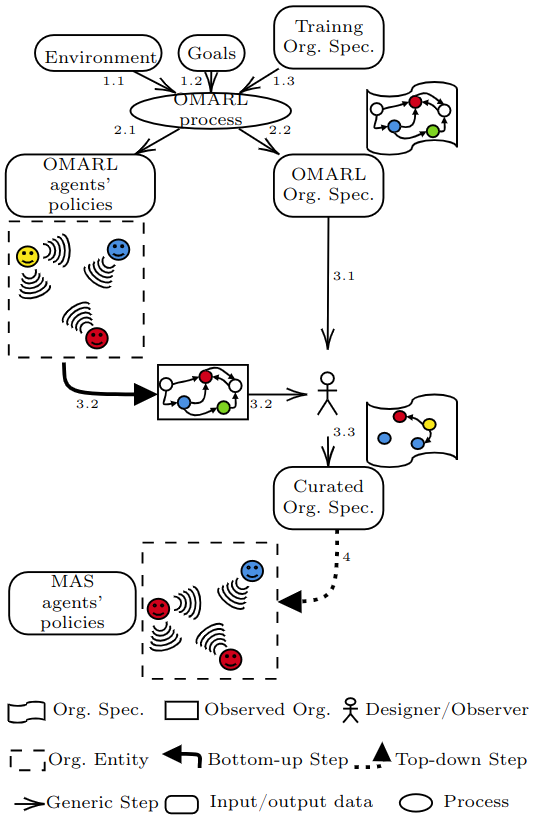
\includegraphics[width=1.2\linewidth]{figures/AOMEA_illustrative_view}
            }
        \end{column}
    
    \end{columns}
    
    \end{frame}    
